\chapter{Model zur Lösung des CSP-Problems}\label{model}

In diesem Kapitel werden anhand von Klassendiagrammen die Bindungs- (Abschnitt \ref{bindunganforderung}) und Routinganforderungen (Abschnitt \ref{routinganforderung}) näher betrachtet. Dabei wird die innere Struktur erläutert, die diese Anforderungen hinzufügen, testen und lösen. Anschließend wird die Implementierung des Min-Conflicts-Embedder (Abschnitt \ref{minConflictImpl}) mit seinen einzelnen Methoden vorgestellt.

\section{Klassendiagramm zum Lösen der Bindungs- und Routinganforderungen}

\subsection{Bindungsanforderungen}\label{bindunganforderung}

Die Abbildung \ref{fig:klBind} zeigt das Klassendiagramm zum Lösen von Bindungsanforderungen. Die Klasse Task speichert in einer Liste alle Bindungsanforderungen (engl. \textit{TaskConstraint}) ab und stellt folgende Funktionen zur Verfügung:

\begin{itemize}
\item \textit{addTaskConstraint}\\
fügt ein Objekt einer abgeleiteten Klasse von \textit{TaskConstraint} der Liste hinzu. 
\item \textit{removeTaskConstraint}\\
löscht ein Objekt vom Typ TaskConstraint aus der Liste.
\item \textit{taskConstraintsAreSatisfied}\\
ruft für alle Objekte in der Liste die Funktion \textit{isSatisfied} aus der Klasse \textit{TaskConstraint} auf. \textit{isSatisfied} überprüft, ob die jeweilige Bindungsanforderung erfüllt ist. Die Funktion gibt \textit{True} zurück, wenn alle Bindungsanforderungen erfüllt sind.%Es wird True zurückgegeben, wenn für alle Objektaufrufe
\item \textit{numberOfFailingConstraint}\\
gibt die Anzahl der fehlgeschlagenen Bindungsanforderungen zurück, wenn man dem Task eine \textit{Unit u} zuweist. 
\item \textit{mapConstraints}\\
weist dem \textit{Task} eine \textit{Unit} zu. Für alle Objekte aus der Liste \textit{list} wird die Methode \textit{map} aufgerufen.
\item \textit{unmapConstraints}\\
entzieht dem Task die \textit{Unit}. Für alle Objekte aus der Liste \textit{list} wird die Methode \textit{unmap} aufgerufen.
\end{itemize}

Um von der abstrakten Klasse \textit{TaskConstraint} zu erben, müssen diese abstrakten Methoden implementiert werden:\\
\begin{itemize}
\item i\textit{sFeasible}\\
überprüft, ob die Anforderung erfüllt wäre, wenn der \textit{Task} auf der \textit{Unit} eingebettet ist. Hierzu wird die Methode \textit{check} mit der Objektvariable der zugehörigen Instanz der Klasse \textit{UnitAttribute} aufgerufen.
\item \textit{isSatisfied}\\
überprüft, ob der eingebettete Task die Anforderung erfüllt. Dazu wird die Methode \textit{check} der zugehörigen \textit{UnitAttribute}-Klasse mit dem Übergabewert \textit{Null} aufgerufen. 
\item \textit{map} \\
ruft bei der zugehörigen \textit{UnitAttribute}-Unterklasse die Methode \textit{update} auf. Der Parameterwert ist die eigene Objektvariable
\item \textit{}unmap\\
ruft bei der zugehörigen \textit{UnitAttribute}-Unterklasse die Methode \textit{update} auf. Der Parameterwert ist der negierte Wert der eigenen Objektvariable
\end{itemize}

Die Klasse \textit{Unit} repräsentiert eine Kachel auf dem Network-on-Chip. Jede Instanz ist durch die Positionsangabe \textit{(x,y)} eindeutig identifizierbar und besitzt eine Liste von Objekten der abgeleiteten Unterklassen der abstrakten Klasse \textit{UnitAttributes}. In der Klasse \textit{Unit} befinden sich folgende Methoden:
\begin{itemize}
\item \textit{addUnitAttriubte}\\
fügt der Liste eine Objekt einer Unterklasse von \textit{UnitAttribute} hinzu.
\item \textit{removeUnitAttriubte}\\
löscht ein Objekt einer Unterklasse von \textit{UnitAttribute} aus der Liste.
\end{itemize}

Eine Kindklasse von \textit{UnitAttribute} muss zwei abstrakten Methoden \textit{check} und \textit{update} implementieren. Jede Kindklasse von \textit{TaskConstraint} verwendet dabei genau einer Kindklasse von \textit{UnitAttribute} und überprüft (\textit{check}) oder aktualisiert (\textit{update}) diese.

\begin{itemize}
\item \textit{check}\\
überprüft, ob es möglich ist, das Attribut zu aktualisieren. D.h. es wird kontrolliert, ob das Objektattribut nach einer Aktualisierung einen gültigen Wert besitzt.
\item \textit{update} \\
aktualisiert die Objektvariable des Attributs.
\end{itemize}

%\todo{TyeAttribute wird nichts upgedated}

\textit{TypeAttribute} ist ein Spezialfall. Hier kann die Objektvariable nicht, wie z. B. bei \textit{UnitWorkloadAttribute}, aktualisiert werden, da der Ressourcentyp sich während der Laufzeit nicht verändern lässt. Deshalb ruft auch die Funktion \textit{update} die Funktion \textit{check} auf und überprüft, ob der gewünschte Ressourcentyp vorliegt.


\begin{figure}[H]\centering
  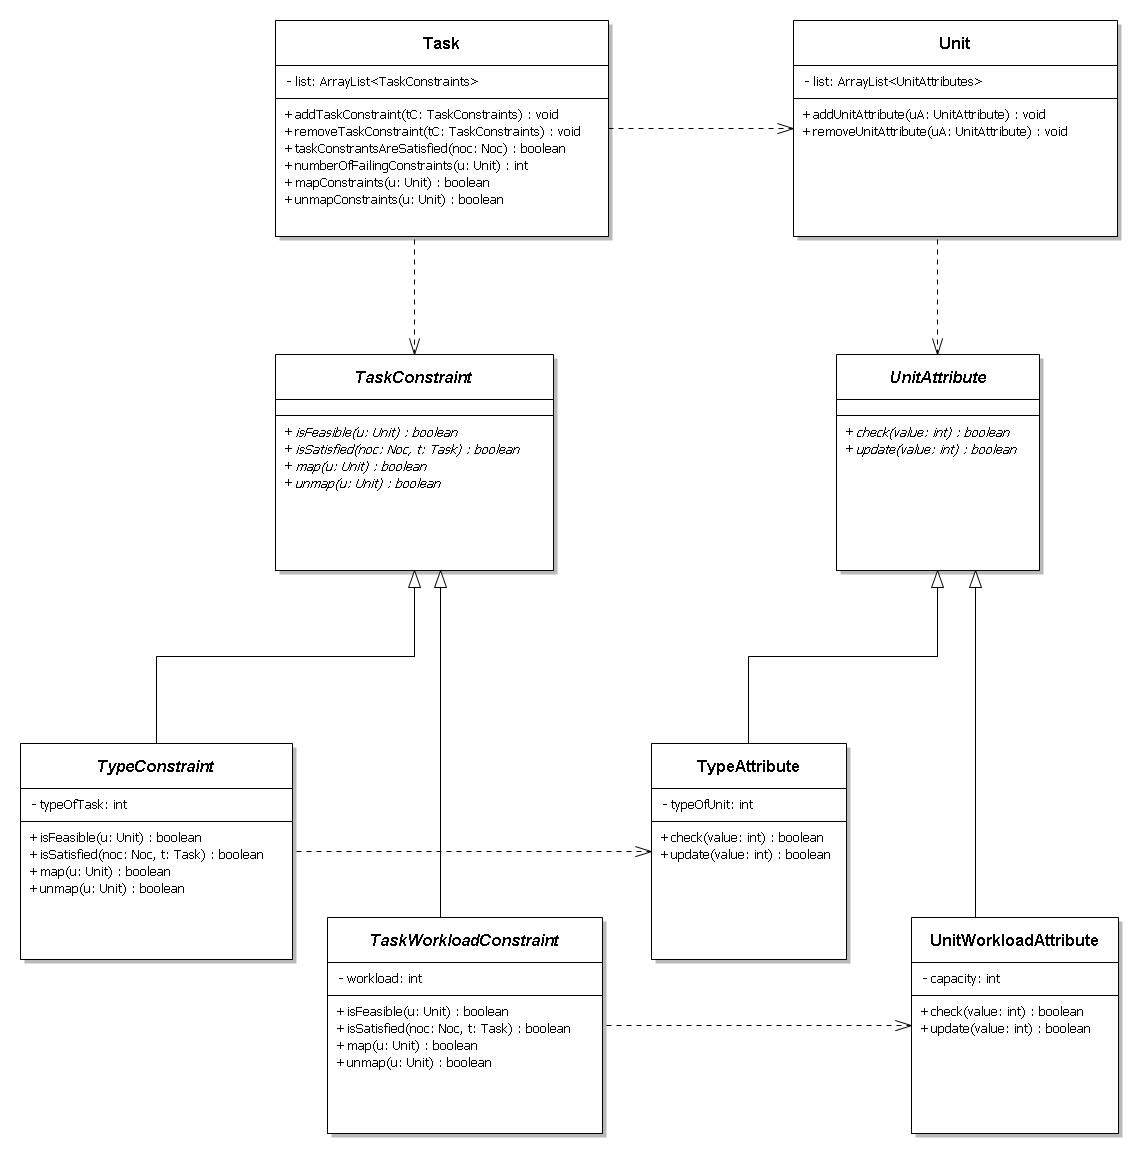
\includegraphics[width = 150mm]{bilder/task-unit.jpg}
  \caption{Klassendiagramm zum Lösen von Bindungsanforderungen}\label{fig:klBind}
\end{figure}

\subsection{Routinganforderungen}\label{routinganforderung}

Das Klassendiagramm zum Lösen von Routinganforderungen (siehe Abbildung \ref{fig:klRoute}) ist dem von Bindungsanforderungen sehr ähnlich. So sind die Methoden und deren Funktionalitäten gleich. Der Unterschied zu den Bindungsanforderungen besteht darin, dass nicht wie bei den Bindungsanforderungen die Attribute von nur einer Kachel (\textit{Unit}) überprüft bzw. aktualisiert werden. Bei den Routinganforderungen werden die Attribute von mehreren \textit{Links}, die zuvor mithilfe eines Routingalgorithmuses ermittelt  wurden, nachgeprüft oder erneuert. \\
\\
Auch hier gibt es mit dem \textit{MaxHopConstraint} einen Spezialfall. Diese Anforderung benötigt kein \textit{LinkAttribute} wie z. B. der  \textit{BandwidthConstraint}, da sie nur überprüft, ob die Anzahl der \textit{Links} in der zuvor berechneten Route eine maximal Anzahl (\textit{maxHops}) nicht überschreitet.
\begin{figure}[H]\centering
  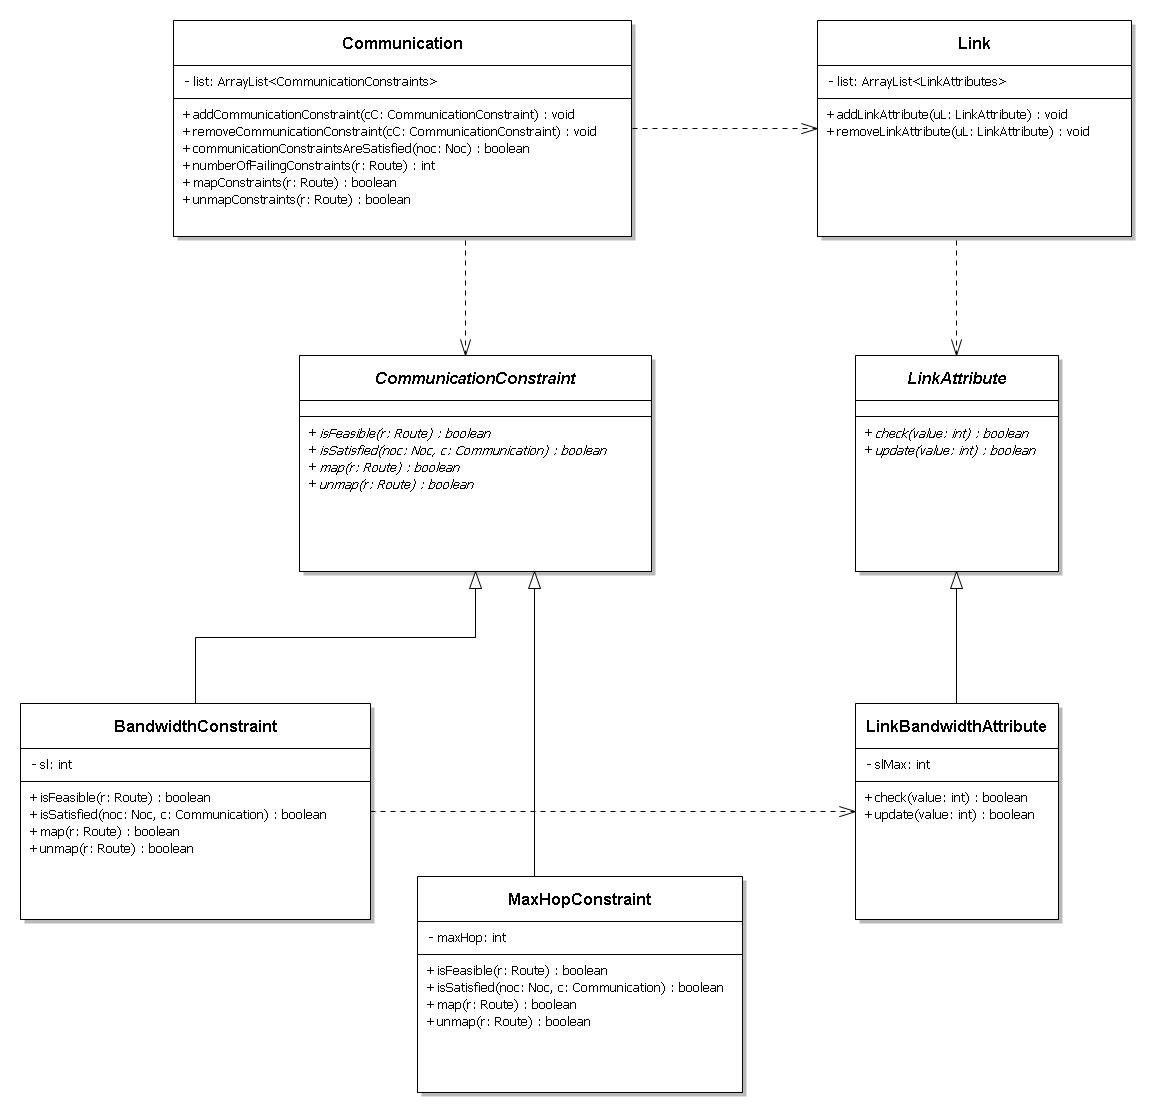
\includegraphics[width = 150mm]{bilder/communication-link.jpg}
  \caption{Klassendiagramm zum Lösen von Routinganforderungen}\label{fig:klRoute}
\end{figure}

\subsection{Hinzufügen von Anforderungen}
Um Anforderungen hinzuzufügen, wird in der Klasse \textit{Task} bzw. \textit{Communication} die Funktion \textit{addTaskConstraint} bzw. \textit{addCommunicationConstraint} aufgerufen. Die Anforderung wir in der ArrayListe \textit{list} gespeichert. Falls eine Anforderung vom gleiche Typ schon vorhanden ist, wird diese durch die neue Anforderung ersetzt. Jede Anforderung (außer der \textit{MaxHopsConstraint}) benötigt ein \textit{Unit-} oder \textit{LinkAttribute}, die beim Konfigurieren des NoCs schon mit \textit{addUnitAttribute} bzw. \textit{addLinkAttribute} hinzugefügt wurde.

\subsection{Überprüfen von Anforderungen}
Um zu überprüfen, ob alle Bindungsanforderungen erfüllt sind, wird in der Klasse \textit{Task} die Methode \textit{taskConstraintsAreSatisfied} aufgerufen. Diese Funktion führt bei jedem Listeneintrag die Funktion \textit{isSatisfied} aus. \textit{isSatisfied} überprüft, ob der Task schon auf eine Kachel des Network-on-Chips eingebettet wurde und ob das dazugehörige \textit{UnitAttribute} einen Fehler meldet.\\
\\
Mit der Funktion \textit{numberOfFailingConstraints} in der Klasse \textit{Task} kann man herausfinden, wie viele Bindungsanforderungen missachtet werden, wenn dem \textit{Task} eine Kachel zugeordnet wird. Hierzu wird für jeden Listeneintrag die \textit{isFeasible}-Methode ausgeführt.\\
\\
Die Überprüfung der Routinganforderungen funktionieren nach dem gleichen Schemata.

\subsection{Zuordnen  von Anforderungen}
Wenn man die Funktion \textit{mapConstraints} in der Klasse \textit{Task} aufruft, werden für alle Listenelemente die Funktion \textit{map} ausgeführt. Diese rufen, die Funktion \textit{update} mit dem Übergabewert der Objektvariable des Listenelements vom dazugehörigen Attribut auf. Dadurch wird die Objektvariable des Attributs aktualisiert.\\
\\
Sollen die Anforderungen wieder entzogen werden, ruft man \textit{unmapConstraints} auf. In dieser Funktion führen alle Listenelemente \textit{unmap} aus. \textit{Unmap} ruft die Funktion \textit{update} des dazugehörigen Attributes auf. Diesmal ist der Übergabewert die negierte Objektvariable des Listenelements.



\section{Implementierung des Min-Conflicts-Embedder}\label{minConflictImpl}

Die Implementierung des Min-Conflicts-Embedder ist anhand des Aktivitätsdiagramm (Abbildung \ref{fig:minConflictsAkti}) graphisch dargestellt. Zuerst wird die Schleifenvariable \textit{j} der äußeren Schleife mit Null initialisiert und die Methode \textbf{mapTaskRandomly} aufgerufen. In \textbf{mapTaskRandomly} wird jedem Task eine zufällig gewählte Kachel, die im Programmcode \textit{Unit} genannt wird, zugeteilt. Es werden dabei Verletzungen der Constraints ignoriert. Anschließend wird der inneren Schleifenvariable \textit{k} dem Wert Null zugewiesen und die Funktion \textbf{findRandomConflictingTask} aufgerufen. Diese Funktion wählt einen Task aus der Menge \textit{C} der Tasks aus, die mindestens einen Constraint verletzen. Falls es keinen Task gibt (\textit{conflictingTask==null}) und somit die Menge \textit{C} leer ist, wurde eine Lösung gefunden (\textbf{success}). Ansonsten wird überprüft, ob die maximale Anzahl an Schleifendurchgängen (\textit{kMax}) erreicht wurde. Wenn dies nicht der Fall ist, ruft das Programm die Funktion \textbf{minConflicts} auf. \textbf{minConflicts} bekommt als Parameter den \textit{conflictingTask} übergeben und versucht für ihn eine geeignete Kachel zu finden, die zu möglichst wenigen Verletzungen einer Bindungs- bzw Routingbedingung führt. Falls es eine derartige Kachel nicht gibt, wird schrittweise der \textit{MaxHopConstraint} gelockert. Das heißt, dass die Manhattan-Distanz schrittweise um eins erhöht wird, bis der Algorithmus eine geeignete Kachel gefunden hat. Ist dies der Fall, wird k inkrementiert und die Funktion \textbf{findRandomConflictingTask} wiederum aufgerufen. \\
\\
Hat \textit{k} den Wert \textit{kMax} erreicht, so ist der Durchgang beendet und alle Tasks werden ihrer Kachel entzogen (\textbf{unmapTasks}). Die Funktion \textbf{mapTaskRandomly} wird aufgerufen und ein neuer Durchgang beginnt. Falls nach \textit{jMax} Durchgängen noch keine Lösung gefunden wurde, beendet sich das Programm (\textbf{fail}).

\begin{figure}[H]\centering
  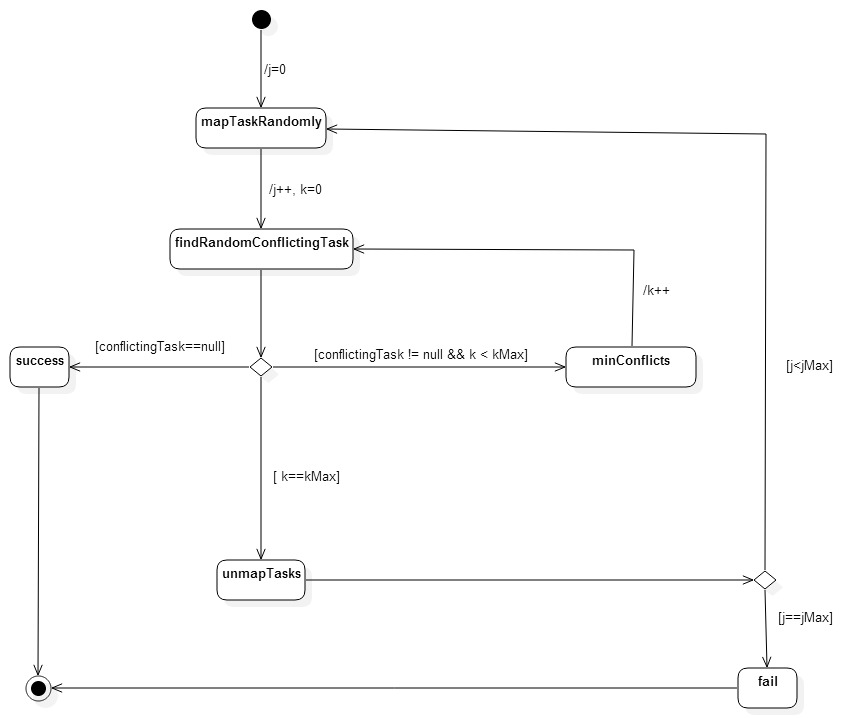
\includegraphics[width = 150mm]{bilder/minAkti.jpg}
  \caption{Das Aktivitätsdiagramm zur Min-Conflicts-Implementierung}\label{fig:minConflictsAkti}
\end{figure}